\documentclass[10pt]{article}

\usepackage[letterpaper,margin=0.5in]{geometry}
\usepackage[T1]{fontenc}
\usepackage[scaled=0.95]{helvet}
\renewcommand{\familydefault}{\sfdefault}
\usepackage{microtype}
\usepackage[table]{xcolor}
\usepackage{graphicx}
\usepackage{tabularx}
\usepackage{array}
\usepackage{booktabs}
\usepackage{enumitem}
\usepackage[most]{tcolorbox}
\usepackage{setspace}

% Agency-style palette and document rhythm.
\definecolor{agencyblue}{HTML}{005A8B}
\definecolor{deepsea}{HTML}{143B5D}
\definecolor{labline}{HTML}{A9BBC8}
\definecolor{panelbg}{HTML}{F6F8FA}
\definecolor{titlebg}{HTML}{EAF2F7}
\definecolor{textgray}{HTML}{2F3B45}

\pagecolor{white}
\pagestyle{empty}
\color{textgray}
\setstretch{0.99}
\setlength{\parindent}{0pt}
\setlength{\parskip}{2.5pt}
\setlength{\tabcolsep}{4pt}
\renewcommand{\arraystretch}{1.08}
\setlist[itemize]{leftmargin=1.15em,labelsep=0.5em,itemsep=2pt,topsep=2pt,parsep=0pt}
\setlist[enumerate]{leftmargin=1.25em,labelsep=0.5em,itemsep=2pt,topsep=2pt,parsep=0pt}
\newcolumntype{Y}{>{\raggedright\arraybackslash}X}

\newtcolorbox{labbox}[2][]{
  colback=panelbg,
  colframe=labline,
  colbacktitle=titlebg,
  coltitle=deepsea,
  fonttitle=\bfseries\small,
  title=\MakeUppercase{#2},
  boxrule=0.5pt,
  arc=0pt,
  left=7pt,
  right=7pt,
  top=5pt,
  bottom=5pt,
  toptitle=3pt,
  bottomtitle=3pt,
  #1
}

\begin{document}
\small

\begin{tcolorbox}[
  colback=white,
  colframe=deepsea,
  boxrule=0.9pt,
  arc=0pt,
  left=8pt,
  right=8pt,
  top=8pt,
  bottom=7pt
]
\begin{minipage}[c]{0.17\textwidth}
\centering
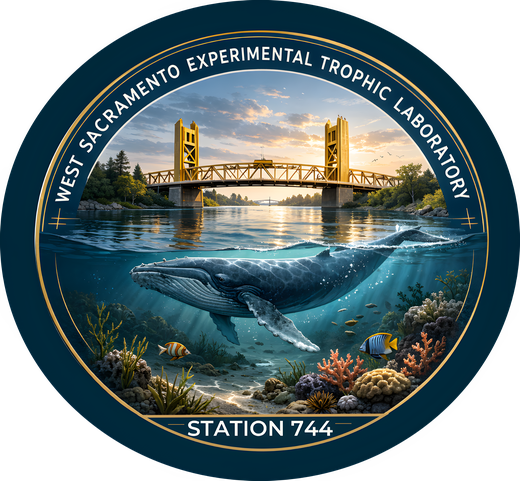
\includegraphics[width=1.00\linewidth]{../images/logo_small.png}
\end{minipage}\hfill
\begin{minipage}[c]{0.78\textwidth}
{\scriptsize\textbf{\color{agencyblue}W.E.T. LAB FIELD OPERATIONS UNIT}}\par
\vspace{2pt}
{\Large\bfseries\color{deepsea}Station 744 Fish Bowl Signal Assay}\par
\vspace{2pt}
{\small Constrained Information Transfer Trial | Semantic Compression Protocol}
\end{minipage}

\vspace{7pt}
{\footnotesize
\rowcolors{1}{titlebg}{white}
\begin{tabularx}{\textwidth}{@{}>{\bfseries\color{deepsea}}l Y >{\bfseries\color{deepsea}}l Y@{}}
Program & Communication ecology and concept transfer testing & Status & Internal use only \\
Study type & Three-round constrained signaling competition & Award & \$300 research funding \\
\end{tabularx}}
\end{tcolorbox}

\vspace{6pt}

\begin{minipage}[t]{0.485\textwidth}
\vspace{0pt}
\begin{labbox}{Study Objective}
Transmit marine species, behaviors, and ecological concepts to your labmates as accurately as possible while the communication channel becomes progressively more restricted.
\end{labbox}

\begin{labbox}{Ecological Background}
\begin{itemize}
\item Marine researchers rarely get perfect observations; identification often relies on a brief sighting, a body posture, or one diagnostic word.
\item Field teams must compress complex observations into signals that remain useful underwater, across distance, or in noisy environments.
\item Efficient communication depends on shared vocabulary, salient traits, and rapid hypothesis narrowing.
\end{itemize}
\end{labbox}

\begin{labbox}{Experimental System}
\begin{itemize}
\item Research lab = team
\item Prompt card = target species, process, or research scenario
\item Clue-giver = signal sender
\item Guessers = receiving analysts
\item Correct guess = successful concept transfer
\item Three rounds = decreasing signal bandwidth
\end{itemize}
\end{labbox}

\begin{labbox}{Protocol}
\begin{enumerate}
\item Two labs compete head-to-head using the marine and science prompt bowl.
\item For each 60-second round, one clue-giver draws prompts one at a time and tries to trigger correct guesses from teammates.
\item Record the number of correct guesses each round, then return all prompts to the bowl before the next round begins.
\item Play the rounds in order: open verbal description, silent acting, then one-word clues. Highest total correct guesses wins the assay.
\end{enumerate}
\end{labbox}
\end{minipage}\hfill
\begin{minipage}[t]{0.485\textwidth}
\vspace{0pt}
\begin{labbox}{Round Constraints}
\begin{tabularx}{\linewidth}{@{}>{\bfseries}l >{\raggedright\arraybackslash}p{0.23\linewidth} Y@{}}
\toprule
Round & Allowed signal & Scientific analog \\
\midrule
1 & Full verbal clues & Describing an organism or event from field notes \\
2 & Silent acting only & Interpreting behavior from motion and posture \\
3 & One-word clue & Diagnostic shorthand used in rapid team communication \\
\bottomrule
\end{tabularx}
\end{labbox}

\begin{labbox}{Prompt Deck Profile}
\begin{itemize}
\item Organism behavior: whale breaching, squid inking, dolphins performing object play.
\item Field science activity: shark tagging, labeling samples, presenting messy data.
\item Ecological stressors: microplastics, entanglement, contamination, predation, bloom events.
\item Absurd but interpretable scenes: reef chaos, grant-writing panic, marine animals behaving badly.
\end{itemize}
\end{labbox}

\begin{labbox}{Scientific Relevance}
This station models how biologists classify and communicate observations under limited information. Teams succeed by selecting diagnostic traits, ecological context, and memorable behaviors that separate one concept from nearby alternatives. The shrinking clue format mimics real research pressure: long-form observation, nonverbal behavior coding, then high-speed shorthand.
\end{labbox}

\begin{labbox}{Observational Notes}
Watch for teams that converge on shared descriptors such as body shape, feeding mode, habitat, or human activity. Strong labs rely on precise ecological cues rather than vague improvisation.
\end{labbox}
\end{minipage}

\vspace{6pt}

\begin{labbox}{Outcome}
Winning lab demonstrates \textbf{superior semantic compression, shared marine vocabulary, and rapid concept classification under constrained signaling}. Award disbursement: \textbf{\$300 research funding}.

\vspace{3pt}
\textbf{Completion bonus reminder:} labs that complete all mini-games earn an additional \textbf{+\$100}.
\end{labbox}

\vfill
\begin{center}
\footnotesize\color{agencyblue}\textbf{W.E.T. LAB | Station 744 | Internal Use Only}
\end{center}

\end{document}
